\documentclass[a4paper,11pt]{article}
\usepackage[a4paper, margin=8em]{geometry}

% usa i pacchetti per la scrittura in italiano
\usepackage[french,italian]{babel}
\usepackage[T1]{fontenc}
\usepackage[utf8]{inputenc}
\frenchspacing 

% usa i pacchetti per la formattazione matematica
\usepackage{amsmath, amssymb, amsthm, amsfonts}

% usa altri pacchetti
\usepackage{gensymb}
\usepackage{hyperref}
\usepackage{standalone}

\usepackage{colortbl}

\usepackage{xstring}
\usepackage{karnaugh-map}

% imposta il titolo
\title{Appunti Sistemi Operativi}
\author{Luca Seggiani}
\date{2025}

% imposta lo stile
% usa helvetica
\usepackage[scaled]{helvet}
% usa palatino
\usepackage{palatino}
% usa un font monospazio guardabile
\usepackage{lmodern}

\renewcommand{\rmdefault}{ppl}
\renewcommand{\sfdefault}{phv}
\renewcommand{\ttdefault}{lmtt}

% circuiti
\usepackage{circuitikz}
\usetikzlibrary{babel}

% testo cerchiato
\newcommand*\circled[1]{\tikz[baseline=(char.base)]{
            \node[shape=circle,draw,inner sep=2pt] (char) {#1};}}

% disponi il titolo
\makeatletter
\renewcommand{\maketitle} {
	\begin{center} 
		\begin{minipage}[t]{.8\textwidth}
			\textsf{\huge\bfseries \@title} 
		\end{minipage}%
		\begin{minipage}[t]{.2\textwidth}
			\raggedleft \vspace{-1.65em}
			\textsf{\small \@author} \vfill
			\textsf{\small \@date}
		\end{minipage}
		\par
	\end{center}

	\thispagestyle{empty}
	\pagestyle{fancy}
}
\makeatother

% disponi teoremi
\usepackage{tcolorbox}
\newtcolorbox[auto counter, number within=section]{theorem}[2][]{%
	colback=blue!10, 
	colframe=blue!40!black, 
	sharp corners=northwest,
	fonttitle=\sffamily\bfseries, 
	title=Teorema~\thetcbcounter: #2, 
	#1
}

% disponi definizioni
\newtcolorbox[auto counter, number within=section]{definition}[2][]{%
	colback=red!10,
	colframe=red!40!black,
	sharp corners=northwest,
	fonttitle=\sffamily\bfseries,
	title=Definizione~\thetcbcounter: #2,
	#1
}

% disponi codice
\usepackage{listings}
\usepackage[table]{xcolor}

\definecolor{codegreen}{rgb}{0,0.6,0}
\definecolor{codegray}{rgb}{0.5,0.5,0.5}
\definecolor{codepurple}{rgb}{0.58,0,0.82}
\definecolor{backcolour}{rgb}{0.95,0.95,0.92}

\lstdefinestyle{codestyle}{
		backgroundcolor=\color{black!5}, 
		commentstyle=\color{codegreen},
		keywordstyle=\bfseries\color{magenta},
		numberstyle=\sffamily\tiny\color{black!60},
		stringstyle=\color{green!50!black},
		basicstyle=\ttfamily\footnotesize,
		breakatwhitespace=false,         
		breaklines=true,                 
		captionpos=b,                    
		keepspaces=true,                 
		numbers=left,                    
		numbersep=5pt,                  
		showspaces=false,                
		showstringspaces=false,
		showtabs=false,                  
		tabsize=2
}

\lstdefinestyle{shellstyle}{
		backgroundcolor=\color{black!5}, 
		basicstyle=\ttfamily\footnotesize\color{black}, 
		commentstyle=\color{black}, 
		keywordstyle=\color{black},
		numberstyle=\color{black!5},
		stringstyle=\color{black}, 
		showspaces=false,
		showstringspaces=false, 
		showtabs=false, 
		tabsize=2, 
		numbers=none, 
		breaklines=true
}


\lstdefinelanguage{assembler}{ 
  keywords={AAA, AAD, AAM, AAS, ADC, ADCB, ADCW, ADCL, ADD, ADDB, ADDW, ADDL, AND, ANDB, ANDW, ANDL,
        ARPL, BOUND, BSF, BSFL, BSFW, BSR, BSRL, BSRW, BSWAP, BT, BTC, BTCB, BTCW, BTCL, BTR, 
        BTRB, BTRW, BTRL, BTS, BTSB, BTSW, BTSL, CALL, CBW, CDQ, CLC, CLD, CLI, CLTS, CMC, CMP,
        CMPB, CMPW, CMPL, CMPS, CMPSB, CMPSD, CMPSW, CMPXCHG, CMPXCHGB, CMPXCHGW, CMPXCHGL,
        CMPXCHG8B, CPUID, CWDE, DAA, DAS, DEC, DECB, DECW, DECL, DIV, DIVB, DIVW, DIVL, ENTER,
        HLT, IDIV, IDIVB, IDIVW, IDIVL, IMUL, IMULB, IMULW, IMULL, IN, INB, INW, INL, INC, INCB,
        INCW, INCL, INS, INSB, INSD, INSW, INT, INT3, INTO, INVD, INVLPG, IRET, IRETD, JA, JAE,
        JB, JBE, JC, JCXZ, JE, JECXZ, JG, JGE, JL, JLE, JMP, JNA, JNAE, JNB, JNBE, JNC, JNE, JNG,
        JNGE, JNL, JNLE, JNO, JNP, JNS, JNZ, JO, JP, JPE, JPO, JS, JZ, LAHF, LAR, LCALL, LDS,
        LEA, LEAVE, LES, LFS, LGDT, LGS, LIDT, LMSW, LOCK, LODSB, LODSD, LODSW, LOOP, LOOPE,
        LOOPNE, LSL, LSS, LTR, MOV, MOVB, MOVW, MOVL, MOVSB, MOVSD, MOVSW, MOVSX, MOVSXB,
        MOVSXW, MOVSXL, MOVZX, MOVZXB, MOVZXW, MOVZXL, MUL, MULB, MULW, MULL, NEG, NEGB, NEGW,
        NEGL, NOP, NOT, NOTB, NOTW, NOTL, OR, ORB, ORW, ORL, OUT, OUTB, OUTW, OUTL, OUTSB, OUTSD,
        OUTSW, POP, POPL, POPW, POPB, POPA, POPAD, POPF, POPFD, PUSH, PUSHL, PUSHW, PUSHB, PUSHA, 
				PUSHAD, PUSHF, PUSHFD, RCL, RCLB, RCLW, MOVSL, MOVSB, MOVSW, STOSL, STOSB, STOSW, LODSB, LODSW,
				LODSL, INSB, INSW, INSL, OUTSB, OUTSL, OUTSW
        RCLL, RCR, RCRB, RCRW, RCRL, RDMSR, RDPMC, RDTSC, REP, REPE, REPNE, RET, ROL, ROLB, ROLW,
        ROLL, ROR, RORB, RORW, RORL, SAHF, SAL, SALB, SALW, SALL, SAR, SARB, SARW, SARL, SBB,
        SBBB, SBBW, SBBL, SCASB, SCASD, SCASW, SETA, SETAE, SETB, SETBE, SETC, SETE, SETG, SETGE,
        SETL, SETLE, SETNA, SETNAE, SETNB, SETNBE, SETNC, SETNE, SETNG, SETNGE, SETNL, SETNLE,
        SETNO, SETNP, SETNS, SETNZ, SETO, SETP, SETPE, SETPO, SETS, SETZ, SGDT, SHL, SHLB, SHLW,
        SHLL, SHLD, SHR, SHRB, SHRW, SHRL, SHRD, SIDT, SLDT, SMSW, STC, STD, STI, STOSB, STOSD,
        STOSW, STR, SUB, SUBB, SUBW, SUBL, TEST, TESTB, TESTW, TESTL, VERR, VERW, WAIT, WBINVD,
        XADD, XADDB, XADDW, XADDL, XCHG, XCHGB, XCHGW, XCHGL, XLAT, XLATB, XOR, XORB, XORW, XORL},
  keywordstyle=\color{blue}\bfseries,
  ndkeywordstyle=\color{darkgray}\bfseries,
  identifierstyle=\color{black},
  sensitive=false,
  comment=[l]{\#},
  morecomment=[s]{/*}{*/},
  commentstyle=\color{purple}\ttfamily,
  stringstyle=\color{red}\ttfamily,
  morestring=[b]',
  morestring=[b]"
}

\lstset{language=assembler, style=codestyle}

% disponi sezioni
\usepackage{titlesec}

\titleformat{\section}
	{\sffamily\Large\bfseries} 
	{\thesection}{1em}{} 
\titleformat{\subsection}
	{\sffamily\large\bfseries}   
	{\thesubsection}{1em}{} 
\titleformat{\subsubsection}
	{\sffamily\normalsize\bfseries} 
	{\thesubsubsection}{1em}{}

% tikz
\usepackage{tikz}

% float
\usepackage{float}

% grafici
\usepackage{pgfplots}
\pgfplotsset{width=10cm,compat=1.9}

% disponi alberi
\usepackage{forest}

\forestset{
	rectstyle/.style={
		for tree={rectangle,draw,font=\large\sffamily}
	},
	roundstyle/.style={
		for tree={circle,draw,font=\large}
	}
}

% disponi algoritmi
\usepackage{algorithm}
\usepackage{algorithmic}
\makeatletter
\renewcommand{\ALG@name}{Algoritmo}
\makeatother

% disponi numeri di pagina
\usepackage{fancyhdr}
\fancyhf{} 
\fancyfoot[L]{\sffamily{\thepage}}

\makeatletter
\fancyhead[L]{\raisebox{1ex}[0pt][0pt]{\sffamily{\@title \ \@date}}} 
\fancyhead[R]{\raisebox{1ex}[0pt][0pt]{\sffamily{\@author}}}
\makeatother

\begin{document}
% sezione (data)
\section{Lezione del 28-10-25}

% stili pagina
\thispagestyle{empty}
\pagestyle{fancy}

% testo
\subsection{Lettori e scrittori}
Sempre sull'argomento della sincronizzazione fra processi, vediamo l'esempio di più \textbf{scrittori} che voglioni scrivere su una risorsa che è letta da più \textbf{lettori}.

Iniziamo a vedere quali politiche vogliamo assicurare:
\begin{enumerate}
	\item Chiaramente, fra gli scrittori c'è una stretta politica di mutua esclusione: non si può scrivere in 2 o più contemporaneamente.
	\item Anche fra lettori e scrittori deve esserci mutua esclusione (non possiamo leggere ciò che è inconsistente perché ci si sta scrivendo);
	\item In tutti gli altri contesti, vorremmo permettere di avere più lettori contemporanei.
\end{enumerate}

Per risolvere il problema della mutua esclusione fra scrittori (1) prevediamo un semaforo di mutex \lstinline|sem wrt = 1|, che viene prelevato in fase di scrittura:
\begin{lstlisting}[language=C++, style=codestyle]	
proc writer {
	wait(wrt); // mutex

	// scrivi

	signal(wrt); // mutex
}
\end{lstlisting}

Il semaforo \lstinline|wrt|, inizialmente pensato per la mutua esclusione fra scrittori (1), può essere usato anche dai lettori per risolvere il problema (2).
Il problema in questo caso sarà che non assicureremo la politica (3) di letture contemporanee: facendo la \lstinline|wait()| su \lstinline|wrt| sblocchiamo infatti un lettore per volta.

Dotiamoci quindi di un contatore \lstinline|int readCount = 0|, che tiene conto dei processi lettori che attualemente stanno leggendo la risorsa.
Proteggiamo quindi il contatore con un nuovo semaforo di mutex \lstinline|sem mutex = 1|.

\begin{lstlisting}[language=C++, style=codestyle]	
proc reader {
	wait(mutex);
	{
		readCount++;
		if(readCount == 1) wait(wrt); // solo il primo aspetta
	}
	signal(mutex);

	// lettura
	
	wait(mutex);
	{
		readCount--;
		if(readCount == 0) signal(wrt); // solo l'ultimo rilascia
	}
	signal(mutex);
}
\end{lstlisting}

In questo caso saranno solo rispettivamente il primo e l'ultimo lettore a prendersi la briga di fare la \lstinline|wait()| e quindi la successiva \lstinline|signal()| sul semaforo condiviso con gli scrittori.

\subsection{Problema dei 5 filosofi}
Veniamo quindi ad un esempio celebre di programmazione concorrente.

\begin{center}
	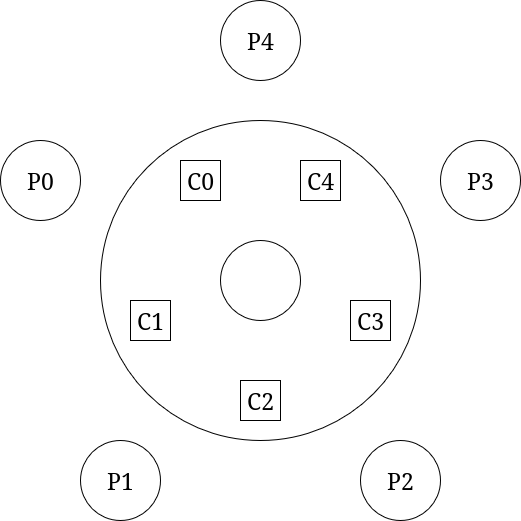
\includegraphics[scale=0.35]{../figures/filosofi.png}
\end{center}

Ipotizziamo una situazione dove 5 filosofi $p_0, p_1, ...$ sono seduti ad una tavola circolare, al centro della quale è posta una scodella di riso. Sulla tavola, una alla destra di ogni filosofo, ci sono esattamente 5 bacchette $c_0, c_1, ...$. Ogni filosofo per mangiare ha bisogno di due bacchette. Il problemaè: come possono i filosofi coordinarsi per mangiare tutti, e quindi ottenere tutti ciclicamente le 2 bacchette?

Contemporaneamente, possono mangiare al massimo 2 filosofi: ad esempio, se sta mangiando $p_0$, possono mangiare contemporaneamente solo $p_2$ o $p_3$.

Vediamo il comportamento del singolo filosofo. Questo potrà trovarsi in uno di 3 stati:
\begin{lstlisting}[language=C++, style=codestyle]	
enum State {
	THINKING, // non ha fame
	HUNGRY,   // sta cercando di ottenere 2 bacchette
	EATING    // sta mangiando
}
\end{lstlisting}

\begin{enumerate}
	\item Un primo approccio può essere quello di dotarsi di un semaforo di mutex per bacchetta, cioè avere \lstinline|sem chopstick[5] = 1|. In questo caso lo pseudocodice del filosofo sarà:
\begin{lstlisting}[language=C++, style=codestyle]	
proc philosopher {
	// pensa

	// aspetta bacchette 
	wait(chopstick[i]); // sx
	wait(chopstick[(i + 1) % 5]); // dx

	// mangia

	// rilascia bacchette
	signal(chopstick[(i + 1) % 5]); // dx
	signal(chopstick[i]); // sx
}
\end{lstlisting}

Questo approccio può però portare a \textit{deadlock} nel caso in cui tutti i processi riescano ad effettuare la prima \lstinline|wait()|: in questo caso si troveranno con la bacchetta a sinistra presa da loro, e quella a destra presa dal vicino, col risultato che nessuno può procedere e i filosofi muoiono di fame. Peccato!

Possiamo modellizzare questa situazione con un grafo, dove nodi circolari rappresentano i \textbf{filosofi} (processi), e nodi quadrati rappresentano le \textbf{bacchette} (\textit{risorse}).
Useremo le frecce da processi e risorse per rappresentare l'\textbf{attesa} di una risorsa (chiamata di \lstinline|wait()|), e le frecce da risorse a processi per rappresentare il \textbf{possesso} di una risorsa (\lstinline|wait()| terminata).

Vediamo che la situazione di deadlock appena descritto in questo caso è rappresentata da un \textbf{ciclo} nel grafo processi-risorse:
\begin{center}
	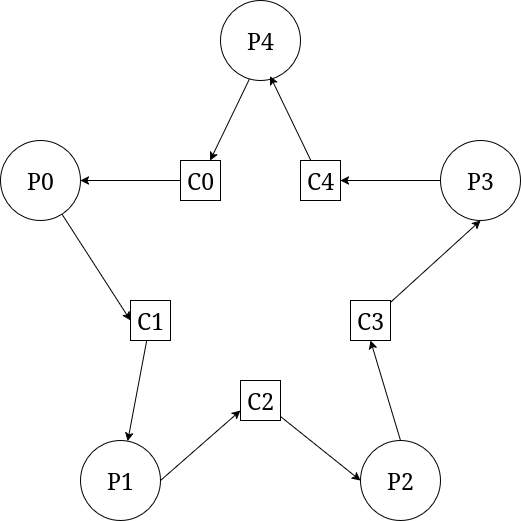
\includegraphics[scale=0.35]{../figures/filosofi_lock.png}
\end{center}

Per risolvere questo problema, vorremo prima approfondire il concetto di deadlock, e quindi implementare appropiate tecniche di deadlock \textbf{detection} (\textit{rilevamento} di deadlock) e deadlock \textbf{avoidance} (\textit{risoluzione} o \textit{prevenzione} di deadlock).
\end{enumerate}

\subsection{Monitor}
I \textbf{monitor} rappresentano un'astrazione di alto livello che permettono la sincronizzazione di processi.
Sostanzialmente, sono strutture dati contenenti funzioni (\textit{operazioni}) che vengono eseguite in mutua esclusione (cioè in maniera \textit{atomica}) all'interno di un certo contesto (dove si condivide codice di \textit{inizializzazione} e \textit{dati}).

All'interno di un monitor prevediamo variabili di \textbf{condizione}, su cui sono permesse operazioni di \lstinline|wait()| e \lstinline|signal()|.
Chiaramente queste variabili di condizioni saranno visibili solo all'\textit{interno} del monitor, cioè del codice delle operazioni definite dal monitor. 

\begin{itemize}
	\item La \lstinline|wait()| mette in attesa un processo finché un altro non esegue una \lstinline|signal()|;
	\item La \lstinline|signal()| sveglia i processi che erano in wait sulla variabile di condizione. La particolarità della \lstinline|signal()| è che non ha effetti se nessuno è in stato di \lstinline|wait()|.
\end{itemize}


\subsubsection{Gestione delle variabili di condizione}
Assumiamo che un processo $P$ invochi \lstinline|x.signal()| sulla variabile di condizione \lstinline|x|, mentre un altro processo $Q$ si trova nello stato \lstinline|x.wait()|. Cosa dovrebbe succedere a questo punto? 

Ci sono due opzioni:
\begin{itemize}
	\item \textbf{Signal and wait}: $P$ aspetta che $Q$ esca dal monitor o si metta in attesa di un'altra condizione: è il caso \textit{preemptive};
	\item \textbf{Signal and continue}: $Q$ aspetta che $P$ esca dal monitor o si metta in attesa di un'altra condizione.
\end{itemize}

Noi adotteremo la soluzione \textit{signal and wait}.

\subsubsection{Monitor per problema dei 5 filosofi}
Vediamo quindi come un monitor può essere usato per risolvere il problema dei 5 filosofi.
\begin{lstlisting}[language=C++, style=codestyle]	
monitor Philosophers {
	enum State {
		THINKING, // non ha fame
		HUNGRY,   // sta cercando di ottenere 2 bacchette
		EATING    // sta mangiando
	}
	State state[5];

	// variabili di condizione
	condition self[5];

	void pickup(int i) {
		state[i] = HUNGRY; // hai fame
		test(i); // puoi mangiare?
		if(state[i] != EATING) self[i].wait(); // se puoi mangia
	}

	void putdown(int i) {
		state[i] = THINKING; // non stai piu' mangiando
		test((i - 1) % 5); // sx puo' mangiare?
		test((i + 1) % 5); // dx puo' mangiare?
	}

	void test(int i) {
		if(
			(state[(i - 1) % 5] != EATING) && // sx non sta mangiando?
			(state[i] == HUNGRY) && 					// hai fame?
			(state[(i + 1) % 5] != EATING)		// dx non sta mangiando?
		) {
			state[i] = EATING; // mangia
			self[i].signal();
		}
	}

	initialization_code() {
		for(int i = 0; i < 5; i++) {
			state[i] = THINKING;
		}
	}
}
\end{lstlisting}

A questo punto il processo filosofo sarà molto semplice:
\begin{lstlisting}[language=C++, style=codestyle]	
process philospher {
	Philosophers.pickup();
	
	// mangia
	
	Philosophers.putdown();
}
\end{lstlisting}

Abbiamo che questo approccio è privo di deadlock. Infatti, i processo filosofi non provano ad ottenere le bacchette finché non hanno la sicurezza di poter prendere \textit{entrambe} le bacchette.

\end{document}
